%!TEX encoding = UTF-8 Unicode
%!TEX root = ../compendium.tex

\Lab{\LabWeekONE}

\begin{Goals}
\item Kunna kombinera principerna sekvens, alternativ, repetition, och abstraktion i skapandet av egna program om minst 20 rader kod.
\item Kunna förklara vad ett program gör i termer av sekvens, alternativ, repetition, och abstraktion.
\item Kunna tillämpa principerna sekvens, alternativ, repetition, och abstraktion i enkla algoritmer.
\item Kunna formatera egna program så att de blir lätta att läsa och förstå.
\item Kunna förklara vad en variabel är och kunna skriva deklarationer och göra tilldelningar.
\item Kunna genomföra upprepade varv i cykeln \emph{editera-exekvera-felsöka/förbättra} för att succesivt bygga upp allt mer utvecklade program.
\end{Goals}

\begin{Preparations}
\item Gör övning {\tt \ExeWeekONE} i kapitel \ref{exe:W01}.
\item Läs igenom ''Kojo - An Introduction'' (25 sidor) som du kan ladda ner i pdf  här: \href{http://www.kogics.net/kojo-ebooks}{http://www.kogics.net/kojo-ebooks}
\item Du behöver en dator med Kojo installerad, se appendix \ref{appendix:kojo}.
\end{Preparations}

\subsection{Obligatoriska uppgifter}


\Task \textit{Sekvens}.

\Subtask Starta Kojo. Om du inte redan har svenska menyer: välj svenska i språkmenyn och starta om Kojo.  Skriv in nedan program och tryck på den \emph{gröna} play-knappen. Du hittar en lista med några fler funktioner på svenska och engelska i appendix \ref{appendix:kojo}.

\begin{Code}
sudda

fram; höger
fram; vänster
\end{Code}


\Subtask Prova att ändra på ordningen mellan satserna och använd den \emph{gula} play-knappen  (programspårning) för att studera vad som händer. Klicka på satser i ditt program och på rutor i programspårningen och se vad som händer.

\Subtask Prova satser i sekvens på flera rader, respektive på samma rad med semikolon emellan. Hur vill du gruppera dina satser så att de är lätta för en människa att läsa?

\Subtask\Pen Vad händer om du \emph{inte} börjar programmet med \code{sudda} och kör det upprepade gånger? Varför är det bra börja programmet med \code{sudda}?

\Subtask Rita en kvadrat som i bilden nedan.

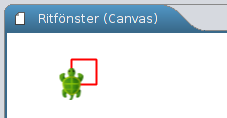
\includegraphics{../img/kojo/kvadrat}

\Subtask Rita en trappa som i bilden nedan.

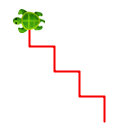
\includegraphics[width=0.25\textwidth]{../img/kojo/stairs}

\Subtask \emph{Rita och mät}.
\begin{itemize}[noitemsep]
\item Börja ditt program med dessa satser:\\ \code{sudda; axesOn; gridOn; sakta(0); osynlig}
\item Rita sedan en kvadrat som har 444 längdenheter i omkrets.
\item Ta fram linjalen med höger-klick i ritfönstret och mät så exakt du kan hur lång diagonalen i kvadraten är. Skriv ner resultatet. \\ \emph{Tips:} Du kan zooma med mushjulet om du håller nere Ctrl-knappen. Du kan flytta linjalen om du klick-drar på linjalens skalstreck. Du kan vrida linjalen om du klickar på skalstrecken och håller nere Shift-tangenten.
\item Kontrollera med hjälp av \code{math.hypot} och \code{println} vad det exakta svaret är. Skriv ner svaret med 3 decimalers noggrannhet.
\end{itemize}

\Subtask Rita en triangel med sidan 300 längdenheter genom att ge lämpliga argument till \code{fram} och \code{höger}. Vinklar anges i grader.

\Subtask\Checkpoint Visa dina resultat för en handledare och diskutera hur uppgifterna ovan illustrerar principen om sekvens.

\Task \textit{Repetition}.

\Subtask Rita en kvadrat igen, men nu med hjälp av proceduren \code+upprepa(n){ ??? }+ där du ersätter \code{n} med antalet repetitioner och ??? med de satser som ska repeteras.

\Subtask Kör ditt program med den \emph{gula} play-knappen. Studera hur repetitionen påverkar  exekveringssekvensen. Vid vilka punkter i programmet sker ett ''hopp'' i sekvensen i stället för att efterföljande sats att exekveras? Använd lämpligt argument till \code{sakta} för att du ska hinna studera exekveringen.

\Subtask Anropa proceduren \code{sakta(???)} med lämplig parameter och gör så att sköldpaddan går totalt 20 varv i kvadraten på ungefär 2 sekunder. \emph{Tips:} Du kan köra ditt program med \emph{Ctrl+Enter} i stället för att trycka på den gröna play-knappen. Anropa \code{sakta} i början av ditt program men \emph{efter} sudda. (Vad händer om du anropar \code{sakta} före \code{sudda}?)


\Subtask Om du anropar \code{sakta(0)}, hur många kvadratvarv hinner sköldpaddan rita på en sekund? Använd nedan program för att ta reda på ungefärligt antal varv per sekund.
\begin{Code}
sudda; sakta(0)
val t1 = System.currentTimeMillis
upprepa(800*4){fram;höger}
val t2 = System.currentTimeMillis
println("Det tog " + (t2 - t1) + " millisekunder")
\end{Code}



\Subtask Rita en kvadrat igen, men nu med hjälp av en \code{while}-sats och en loop-variabel.

\begin{Code}
var i = 0
while (???) {fram; höger; i = ???}
\end{Code}

\Subtask Rita en kvadrat igen, men nu med hjälp av en \code{for}-sats.

\begin{Code}
for (i <- 1 to ???) {???}
\end{Code}

\Subtask Rita en kvadrat igen, men nu med hjälp av \code{foreach}.

\begin{Code}
(1 to ???).foreach{i => ???}
\end{Code}


\Subtask\Checkpoint Vad är fördelar och nackdelar med de olika sätten att loopa: \code{upprepa}, \code{while}, \code{for}, respektive \code{foreach}? \Pen Diskutera dina svar med en handledare.

\Task \textit{Abstraktion}.

\Subtask Använd en repetition för abstrahera nedan sekvens, så att programmet blir kortare:
\begin{Code}
sudda

fram; höger; hoppa; fram; vänster; hoppa; fram; höger;
hoppa; fram; vänster; hoppa; fram; höger; hoppa; fram;
vänster; hoppa; fram; höger; hoppa; fram; vänster; hoppa;
fram; höger; hoppa; fram; vänster; hoppa
\end{Code}

\Subtask\Pen Sök på nätet efter ''DRY principle programming'' och beskriv med egna ord vad DRY betyder och varför det är en viktig princip.

\Subtask Använd proceduren \code{kvadrat} nedan och proceduren \code{hoppa(???)} för att rita en stapel med 10 kvadrater enligt bilden.

\begin{Code}
def kvadrat = for (i <- 1 to 4) {fram; höger}
\end{Code}

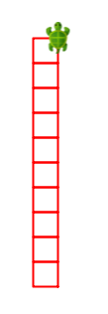
\includegraphics[scale=0.5]{../img/kojo/square-column}

\Subtask Kör ditt program med den \emph{gula} play-knappen. Studera hur anrop av proceduren \code{kvadrat} påverkar exekveringssekvensen av dina satser. Vid vilka punkter i programmet sker ett ''hopp'' i sekvensen i stället för att efterföljande sats att exekveras? Använd lämpligt argument till \code{sakta} för att du ska hinna studera exekveringen.

\Subtask Rita samma bild med 10 staplade kvadrater som ovan, men nu \emph{utan} att använda abstraktionen \code{kvadrat} -- använd i stället en nästlad repetition. Vilket av de två sätten (med och utan abstraktionen \code{kvadrat}) är lättast att läsa?\\ \emph{Tips:} Varje gång du trycker på någon av play-knapparna, sparas ditt program. Du kan se dina sparade program om du klickar på \emph{Historik}-fliken. Du kan också stega bakåt och framåt i historiken med de blå pilarna bredvid play-knapparna.

\Subtask Skapa en abstraktion \code{def stapel = ???} med din kod för att rita en stapel.

\Subtask Du ska nu generalisera din procedur så att den inte bara kan rita exakt 10 kvadrater i en stapel. Ge proceduren \code{stapel} en parameter \code{n} som styr hur många kvadrater som ritas.
\begin{Code}
def kvadrat = ???
def stapel(n: Int) = ???

sudda; sakta(100)
stapel(42)
\end{Code}

\Subtask Ge abstraktionen \code{kvadrat} en parameter \code{sida: Double} som anger hur stor kvadraten blir. Rita flera kvadrater i likhet med bilden nedan.

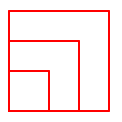
\includegraphics{../img/kojo/square-param}

\Subtask Rita nedan bild med hjälp av abstraktionen \code{stapel}. Det är totalt 100 kvadrater och varje kvadrat har sidan 25. \emph{Tips:} Med ett negativt argument till procedur \code{hoppa} kan du få sköldpaddan att hoppa baklänges utan att rita, t.ex. \code{hoppa(-10*25)}

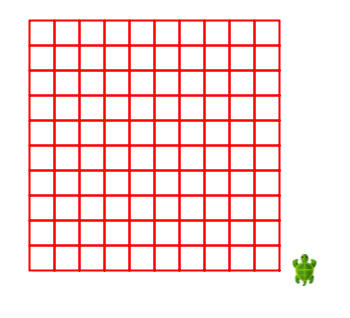
\includegraphics[width=0.3\textwidth]{../img/kojo/square-grid}

\Subtask Skapa en abstraktion \code{rutnät} med lämpliga parametrar som gör att man kan rita rutnät med olika stora kvadrater och olika många kvadrater i både x- och y-led.

\Subtask\Checkpoint Se över ditt program i föregående uppgift och säkerställ att det är lättläst och följer en struktur som börjar med alla definitioner i logisk ordning och därefter fortsätter med huvudprogrammet. Diskutera ditt program med en handledare. Vad har du gjort för att programmet ska vara lättläst?


\Task \emph{Variabel.}

\Subtask Skriv in nedan program \emph{exakt} som det står med blanktecken, indragningar och radbrytningar. Kör programmet och förklara vad som händer.

\begin{Code}
def gurka(x: Double,
          y: Double, namn: String,
          typ: String,
          värde:String) = {
  val bredd = 15
  val h = 30
  hoppaTill(x,y)
  norr
  skriv(namn+": "+typ)
  hoppaTill(x+bredd*(namn.size+typ.size),y)
  skriv(värde); söder; fram(h); vänster
  fram(bredd * värde.size); vänster
  fram(h); vänster
  fram(bredd * värde.size); vänster
}

sudda; färg(svart)
val s = 130
val h = 40
var x = 42; gurka(10, s-h*0, "x","Int", x.toString)
var y = x;  gurka(10, s-h*1, "y","Int", y.toString)
x = x + 1;  gurka(10, s-h*2, "x","Int", x.toString)
            gurka(10, s-h*3, "y","Int", y.toString)
osynlig
\end{Code}

\Subtask\Pen Skriv ner namnet på alla variabler som förekommer i programmet ovan.

\Subtask\Pen Vilka av dessa variabler är lokala?

\Subtask\Pen Vilka av dessa variabler kan förändras?

\Subtask\Pen Föreslå tre förändringar av programmet ovan (till exempel namnbyten) som gör att det blir lättare att läsa och förstå.

\Subtask Gör sök-ersätt av \code{gurka} till ett bättre namn. \emph{Tips:} undersök kontextmenyn i editorn i Kojo genom att högerklicka i editorfönstret. Notera kortkommandot för Sök/Ersätt.

\Subtask\Checkpoint Gör automatisk formatering av koden med hjälp av lämpligt editor-kortkommando. Notera skillnaderna. Vilka autoformateringar gör programmet lättare att läsa? Vilka manuella formateringar tycker du bör göras för att öka läsbarheten? Diskutera läsbarheten med en handledare.

\Task \emph{Alternativ.}

\Subtask Kör programmet nedan. Förklara vad som händer. Använd den gula play-knappen för att studera exekveringen.

\begin{Code}
sudda; sakta(5000)

def move(key: Int): Unit = {
  println("key: " + key)
  if (key == 87) fram(10)
  else if (key == 83) fram(-10)
}

move(87); move('W'); move('W')
move(83); move('S'); move('S'); move('S')
\end{Code}

\Subtask Kör programmet nedan. Notera \code{activateCanvas} för att du ska slippa klicka i ritfönstret innan du kan styra paddan. Lägg till kod i \code{move} som gör att tangenten A ger en vridning moturs med 5 grader medan tangenten D ger en vridning medurs 5 grader.

\begin{Code}
sudda; sakta(0); activateCanvas

def move(key: Int): Unit = {
  println("key: " + key)
  if (key == 'W') fram(10)
  else if (key == 'S') fram(-10)
}

onKeyPress(move)
\end{Code}

\Subtask Lägg till nedan kod i början av programmet och gör så att när man trycker på tangenten G så sätter man omväxlande på och av rutnätet.

\begin{Code}
var isGridOn = false

def toggleGrid =
  if (isGridOn) {
    gridOff
    isGridOn = false
  } else {
    gridOn
    isGridOn = true
  }
\end{Code}

\Subtask\Checkpoint Gör så att när man trycker på tangenten X så sätter man omväxlande på och av koordinataxlarna. Använd en variabel \code{isAxesOn} och definiera en abstraktion \code{toggleAxes} som anropar \code{axesOn} och \code{axesOff} på liknande sätt som i föregående uppgift. Visa din lösning för en handledare.

\subsection{Frivilliga extrauppgifter}

\Task \emph{Tidmätning.} Hur snabb är din dator?

\Subtask \label{task:timer} Skriv in koden nedan i Kojos editor och kör upprepade gånger med den gröna play-knappen. Hur lång tid tar det för din dator att räkna till 4.4 miljarder?\footnote{Det går att göra ungefär en heltalsaddition per klockcykel per kärna. Den första elektroniska datorn Eniac hade en klockfrekvens motsvarande 5kHz. Björn Regnells dator har en i7-4790K som turboklockar på 4.4 GHz.

\href{http://www.extremetech.com/computing/185512-overclocking-intels-core-i7-4790k-can-devils-canyon-fix-haswells-low-clock-speeds/2}{www.extremetech.com/computing/185512-overclocking-intels-core-i7-4790k-can-devils-canyon-fix-haswells-low-clock-speeds/2}
}

\begin{Code}
object timer {
  def now: Long = System.currentTimeMillis
  var saved: Long = now
  def elapsedMillis: Long = now - saved
  def elapsedSeconds: Double = elapsedMillis / 1000.0
  def reset: Unit = { saved = now }
}

// HUVUDPROGRAM:
timer.reset
var i = 0L
while (i < 1e8.toLong) { i += 1 }
val t = timer.elapsedSeconds
println("Räknade till " + i + " på " + t + " sekunder.")
\end{Code}

\Subtask  Om du kör på en Linux-maskin: Kör nedan Linux-kommando upprepade gånger i ett terminalfönster. Med hur många MHz kör din dators klocka för tillfället? Hur förhåller sig klockfrekvensen till antalet rundor i while-loopen i föregående uppgift? (Det kan hända att din dator kan variera centralprocessorns klockfrekvens. Prova både medan du kör tidmätningen i Kojo och då din dator ''vilar''. Vad är det för poäng med att en processor kan variera sin klockfrekvens?)
\begin{REPL}
> lscpu | grep MHz
\end{REPL}


\Subtask Ändra i koden i uppgift \ref{task:timer}) så att \code{while}-loopen bara kör 5 gånger. Kör programmet med den \emph{gula} play-knappen. Scrolla i programspårningen och förklara vad som händer. Klicka på \code{CALL}-rutorna och se vilken rad som markeras i ditt program.

\Subtask Lägg till koden nedan i ditt program och försök ta reda på ungefär hur långt din dator hinner räkna till på en sekund för \code{Long}- respektive \code{Int}-variabler. Använd den gröna play-knappen.
\begin{Code}
def timeLong(n: Long): Double = {
  timer.reset
  var i = 0L
  while (i < n) { i += 1 }
  timer.elapsedSeconds
}

def timeInt(n: Int): Double = {
  timer.reset
  var i = 0
  while (i < n) { i += 1 }
  timer.elapsedSeconds
}

def show(msg: String, sec: Double): Unit = {
  print(msg + ": ")
  println(sec + " seconds")
}

def report(n: Long): Unit = {
  show("Long " + n, timeLong(n))
  if (n <= Int.MaxValue) show("Int  " + n, timeInt(n.toInt))
}

// HUVUDPROGRAM, mätningar:

report(Int.MaxValue)

for (i <- 1 to 10) {
  report(4.26e9.toLong)
}
\end{Code}

\Subtask\Checkpoint Hur mycket snabbare går det att räkna med \code{Int}-variabler jämfört med \code{Long}-variabler? Visa svaret för en handledare.

\Task Lek med färg i Kojo. Sök på internet efter dokumentationen för klassen java.awt.Color och studera vilka heltalsparametrar den sista konstruktorn i listan med konstruktorer tar för att skapa sRGB-färger. Om du högerklickar i editorn i Kojo och väljer ''Välj färg...'' får du fram färgväljaren.

\begin{REPL}
scala> val c = new java.awt.Color(124,10,78,100)
c: java.awt.Color = java.awt.Color[r=124,g=10,b=78]

scala> c.  // tryck på TAB
asInstanceOf    getColorComponents      getRGBComponents
brighter        getColorSpace           getRed
createContext   getComponents           getTransparency
darker          getGreen                isInstanceOf
getAlpha        getRGB                  toString
getBlue         getRGBColorComponents

scala> c.getAlpha
res3: Int = 100
\end{REPL}

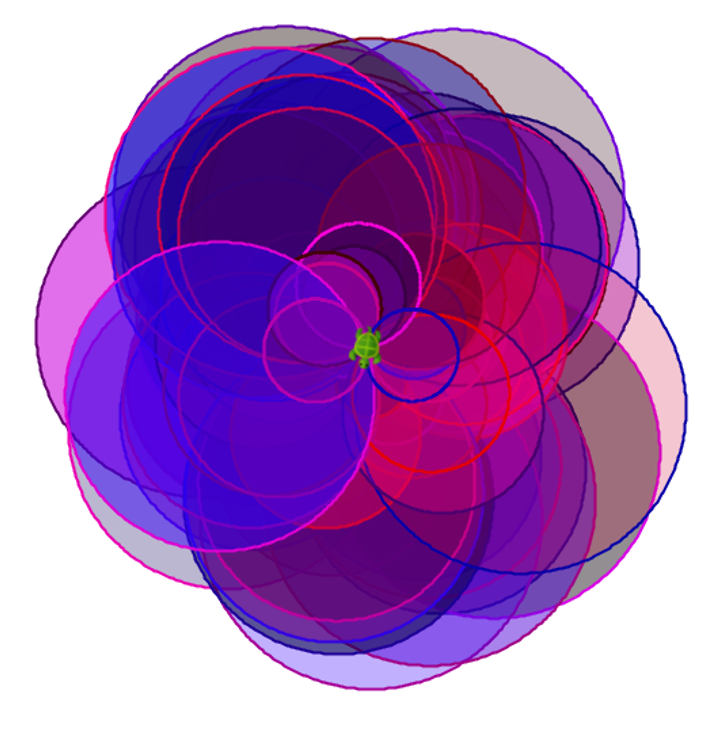
\includegraphics[width=0.75\textwidth]{../img/kojo/random-color-circles.png}


\Task Ladda ner dessa pdf-kompendier och gör några uppgifter som du tycker verkar intressanta:

\Subtask ''Uppdrag med Kojo'' som kan laddas ner här:\\ \href{http://fileadmin.cs.lth.se/cs/Personal/Bjorn_Regnell/uppdrag.pdf}{fileadmin.cs.lth.se/cs/Personal/Bjorn\_Regnell/uppdrag.pdf}

\Subtask ''Programming Fundamentals with Kojo'' som kan laddas ner här:\\
 \href{http://wiki.kogics.net/kojo-codeactive-books}{wiki.kogics.net/kojo-codeactive-books}
